\documentclass[xetex,14pt,aspectratio=169]{beamer}

\usepackage{caption}
\usepackage[percent]{overpic}
\usepackage{xecyr}
\usepackage{xunicode}
\usepackage[absolute,overlay]{textpos}
\usepackage{fontspec}
\usepackage{calc}
\usepackage{multicol}
\usepackage{hyperref}
\usepackage{setspace}
\defaultfontfeatures{Ligatures=TeX}
\setmainfont{Microsoft Sans Serif}
\usepackage{polyglossia}
\setdefaultlanguage[spelling=modern]{russian}
\newfontfamily{\cyrillicfont}{Microsoft Sans Serif}
\newfontfamily{\cyrillicfontsf}{Microsoft Sans Serif}
\newfontfamily{\cyrillicfonttt}{Microsoft Sans Serif}

\mode<presentation>
{
  \usetheme{Boadilla}      % or try Darmstadt, Madrid, Warsaw, ...
  \usecolortheme{default} % or try albatross, beaver, crane, ...
  \usefonttheme{default}  % or try serif, structurebold, ...
  \setbeamertemplate{navigation symbols}{}
  \setbeamertemplate{caption}[numbered]
  \setbeamertemplate{itemize items}[circle]
  \setbeamerfont{title}{series=\bfseries,parent=structure}
} 

\makeatother
\setbeamertemplate{footline}
{
  \leavevmode%
  \hbox{%
  \begin{beamercolorbox}[wd=.4\paperwidth,ht=2.5ex,dp=1ex,center]{author in head/foot}%
    \usebeamerfont{author in head/foot}\insertshortauthor
  \end{beamercolorbox}%
  \begin{beamercolorbox}[wd=.6\paperwidth,ht=2.5ex,dp=1ex,center]{title in head/foot}%
    \usebeamerfont{title in head/foot}\insertshorttitle\hfill
    \insertframenumber{} / \inserttotalframenumber\hspace*{-8ex}
  \end{beamercolorbox}}%
  \vskip0pt%
}
\makeatletter

\title[Gathering and visualizing flamegraphs in realtime]{On performance analyzing again:\\ {Gathering and visualizing flamegraphs in realtime in Linux environment}}
\author[Alex Chistyakov, DataArt]{Alex Chistyakov, DataArt}
\institute[]{Linux Piter 2016, Russia, SPb.}
\date{}

\begin{document}

\setlength{\fboxsep}{0pt}

\begin{frame}
  \titlepage
\end{frame}

\begin{frame}{Who I am (very quickly)}
\setstretch{1.2}
\begin{textblock*}{\framewidth-0.8cm}(0.0cm,1.5cm) % {block width} (coords)
\begin{itemize}
  \item Senior SW Developer @ DataArt
  \item More than 18 years of professional experience
  \item Researcher @ ISST Lab, ITMO
  \item Used to be a DevOps Engineer and still probably am
  \item Can't quit making presentations w/lots of bullets (that's terrible, I know)
\end{itemize}
\end{textblock*}
\end{frame}

\begin{frame}{Performance optimization is not that hard}
\setstretch{1.2}
\begin{textblock*}{\framewidth-0.8cm}(0.0cm,1.5cm) % {block width} (coords)
\begin{minipage}{\textwidth}
  \centering
  
\includegraphics[width=8cm]{img/owl}
\end{minipage}
\end{textblock*}
\end{frame}

\begin{frame}{Ever heard of a 'comfort zone'?}
\setstretch{1.2}
\begin{textblock*}{\framewidth-0.8cm}(0.0cm,1.5cm) % {block width} (coords)
\begin{itemize}
  \item It's crucial to be out of it to learn something new
\end{itemize}
\end{textblock*}
\end{frame}

\begin{frame}{Ever heard of a 'comfort zone'?}
\setstretch{1.2}
\begin{textblock*}{\framewidth-0.8cm}(0.0cm,1.5cm) % {block width} (coords)
\begin{itemize}
  \item It's crucial to be out of it to learn something new
  \item So I made this presentation in TeX
\end{itemize}
\end{textblock*}
\end{frame}

\begin{frame}{Ever heard of a 'comfort zone'?}
\setstretch{1.2}
\begin{textblock*}{\framewidth-0.8cm}(0.0cm,1.5cm) % {block width} (coords)
\begin{itemize}
  \item It's crucial to be out of it to learn something new
  \item So I made this presentation in TeX
  \item With lots of bullets, you know
\end{itemize}
\end{textblock*}
\end{frame}

\begin{frame}{Ever heard of a 'comfort zone'?}
\setstretch{1.2}
\begin{textblock*}{\framewidth-0.8cm}(0.0cm,1.5cm) % {block width} (coords)
\begin{itemize}
  \item It's crucial to be out of it to learn something new
  \item So I made this presentation in TeX
  \item With lots of bullets, you know
  \item Because I'm not ready yet to leave my comfort zone entirely
\end{itemize}
\end{textblock*}
\end{frame}

\begin{frame}{Ever heard of a 'comfort zone'?}
\setstretch{1.2}
\begin{textblock*}{\framewidth-0.8cm}(0.0cm,1.5cm) % {block width} (coords)
\begin{itemize}
  \item It's crucial to be out of it to learn something new
  \item So I made this presentation in TeX
  \item With lots of bullets, you know
  \item Because I'm not ready yet to leave my comfort zone entirely
  \item Damn, TeX seems to be my new comfort zone ;(
\end{itemize}
\end{textblock*}
\end{frame}

\begin{frame}{Okay, flashback to LP 2015 (w/no bullets)}
\setstretch{1.2}
\begin{textblock*}{\framewidth-0.8cm}(0.0cm,1.5cm) % {block width} (coords)
\begin{minipage}{\textwidth}
  \centering
  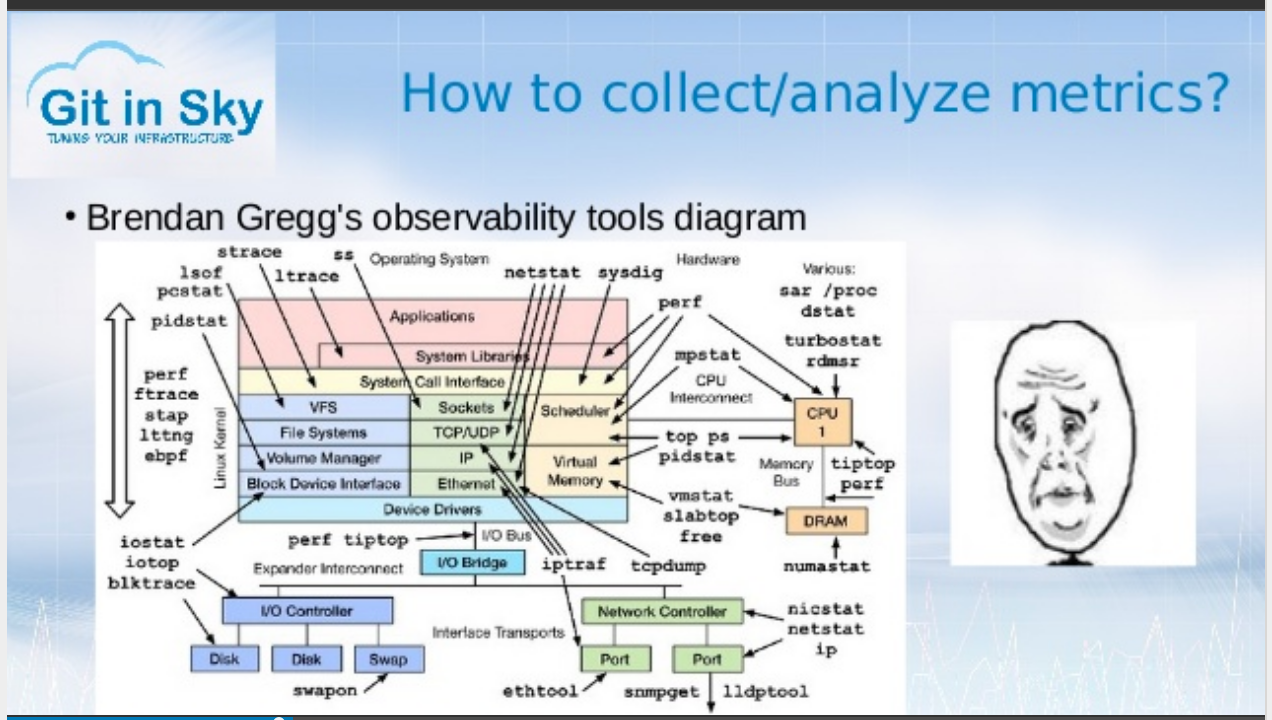
\includegraphics[height=7cm]{img/2015.png}
\end{minipage}
\end{textblock*}
\end{frame}

\begin{frame}{Fast-forward to 2016}
\setstretch{1.2}
\begin{textblock*}{\framewidth-0.8cm}(0.7cm,1.5cm) % {block width} (coords)
Brendan Gregg declared Linux DTrace-complete!
\begin{minipage}{\textwidth}
  \centering
  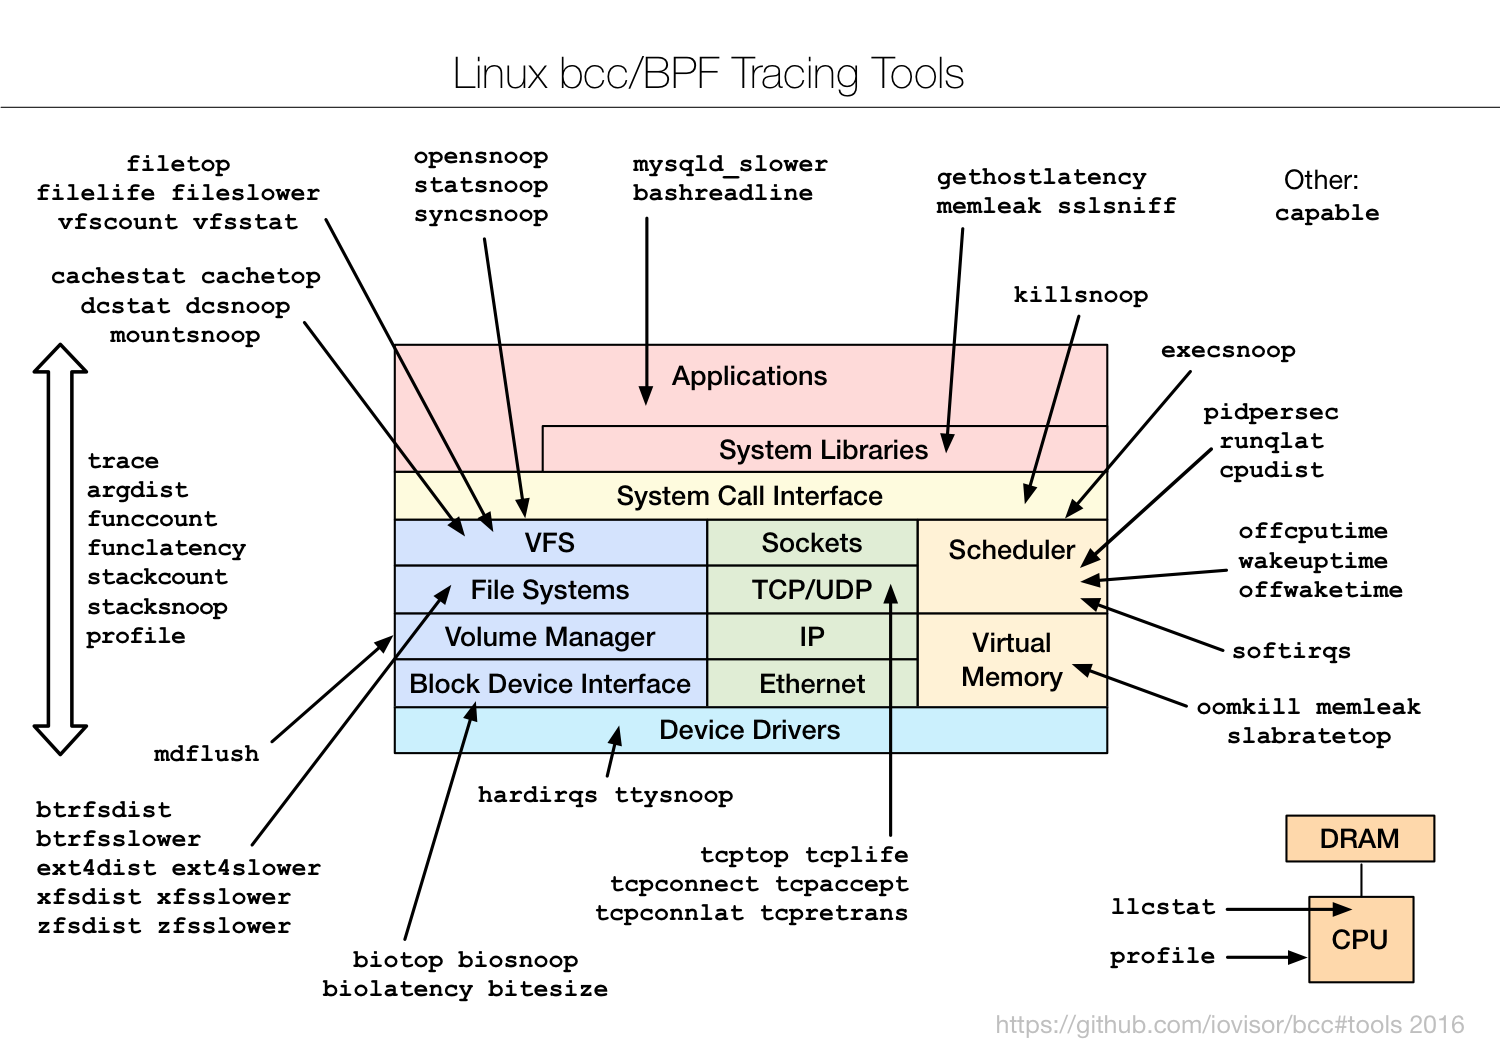
\includegraphics[height=6.6cm]{img/2016.png}
\end{minipage}
\end{textblock*}
\end{frame}

\begin{frame}{A great step forward for mankind...}
\setstretch{1.2}
\begin{textblock*}{\framewidth-0.8cm}(0.7cm,1.5cm) % {block width} (coords)
...but I'm a cat
\begin{minipage}{\textwidth}
  \centering
  
\includegraphics[height=6.6cm]{img/cat}
\end{minipage}
\end{textblock*}
\end{frame}

\begin{frame}{So, what is this all about?}
\setstretch{1.2}
\begin{textblock*}{\framewidth-0.8cm}(0.0cm,1.5cm) % {block width} (coords)
\begin{itemize}
  \item Modern GNU/Linux
\end{itemize}
\end{textblock*}
\end{frame}

\begin{frame}{So, what is this all about?}
\setstretch{1.2}
\begin{textblock*}{\framewidth-0.8cm}(0.0cm,1.5cm) % {block width} (coords)
\begin{itemize}
  \item Modern GNU/Linux
  \item A web application
\end{itemize}
\end{textblock*}
\end{frame}

\begin{frame}{So, what is this all about?}
\setstretch{1.2}
\begin{textblock*}{\framewidth-0.8cm}(0.0cm,1.5cm) % {block width} (coords)
\begin{itemize}
  \item Modern GNU/Linux
  \item A web application
  \item Collecting flamegraphs
\end{itemize}
\end{textblock*}
\end{frame}

\begin{frame}{So, what is this all about?}
\setstretch{1.2}
\begin{textblock*}{\framewidth-0.8cm}(0.0cm,1.5cm) % {block width} (coords)
\begin{itemize}
  \item Modern GNU/Linux
  \item A web application
  \item Collecting flamegraphs
  \item Visualizing collected flamegraphs
\end{itemize}
\end{textblock*}
\end{frame}

\begin{frame}{Okay, but what are these flame... things?}
\setstretch{1.2}
\begin{textblock*}{\framewidth-0.8cm}(0.7cm,1.5cm) % {block width} (coords)
Did you attend LP 2015?
\begin{minipage}{\textwidth}
  \centering
  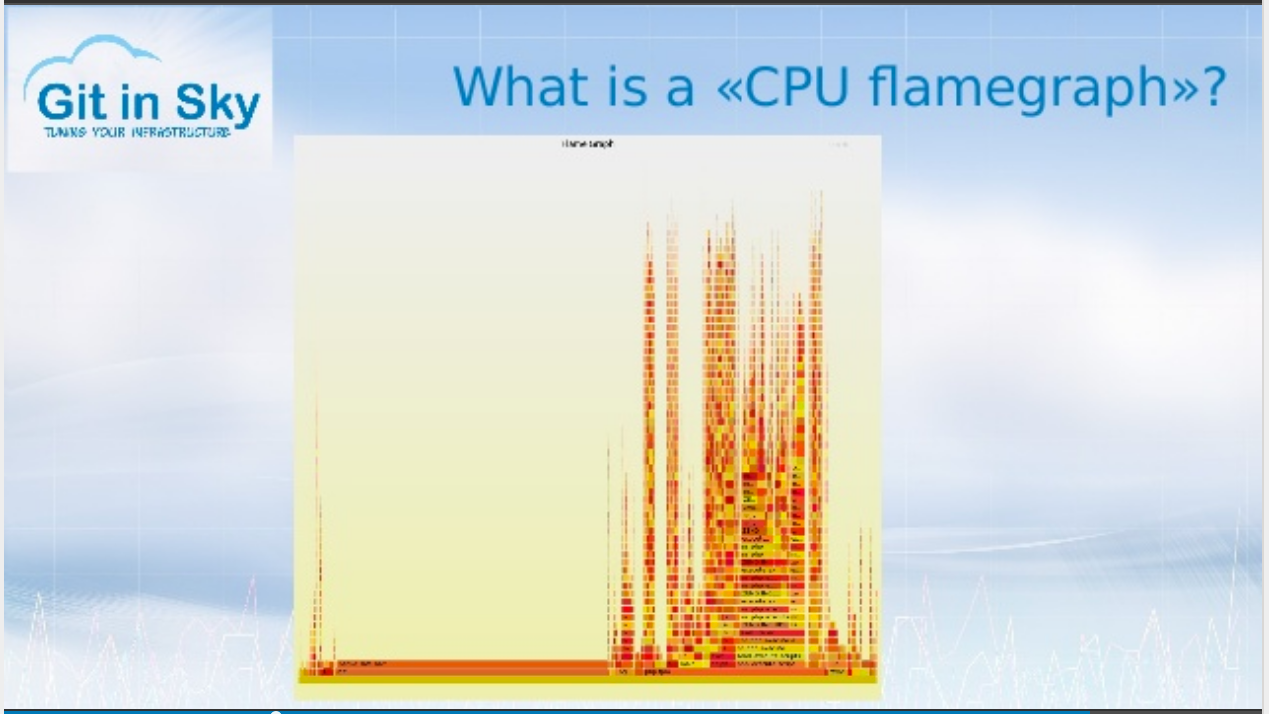
\includegraphics[height=6.6cm]{img/2015-fg.png}
\end{minipage}
\end{textblock*}
\end{frame}

\begin{frame}{Doing flamegraphs in 2016 is extremely easy}
\setstretch{1.2}
\begin{textblock*}{\framewidth-0.8cm}(0.0cm,1.5cm) % {block width} (coords)
\begin{minipage}{\textwidth}
  \centering
  
\includegraphics[width=8cm]{img/owl}
\end{minipage}
\end{textblock*}
\end{frame}

\begin{frame}{A hicker needs good boots}
\setstretch{1.2}
\begin{textblock*}{\framewidth-0.8cm}(0.0cm,1.5cm) % {block width} (coords)
\begin{minipage}{\textwidth}
  \centering
  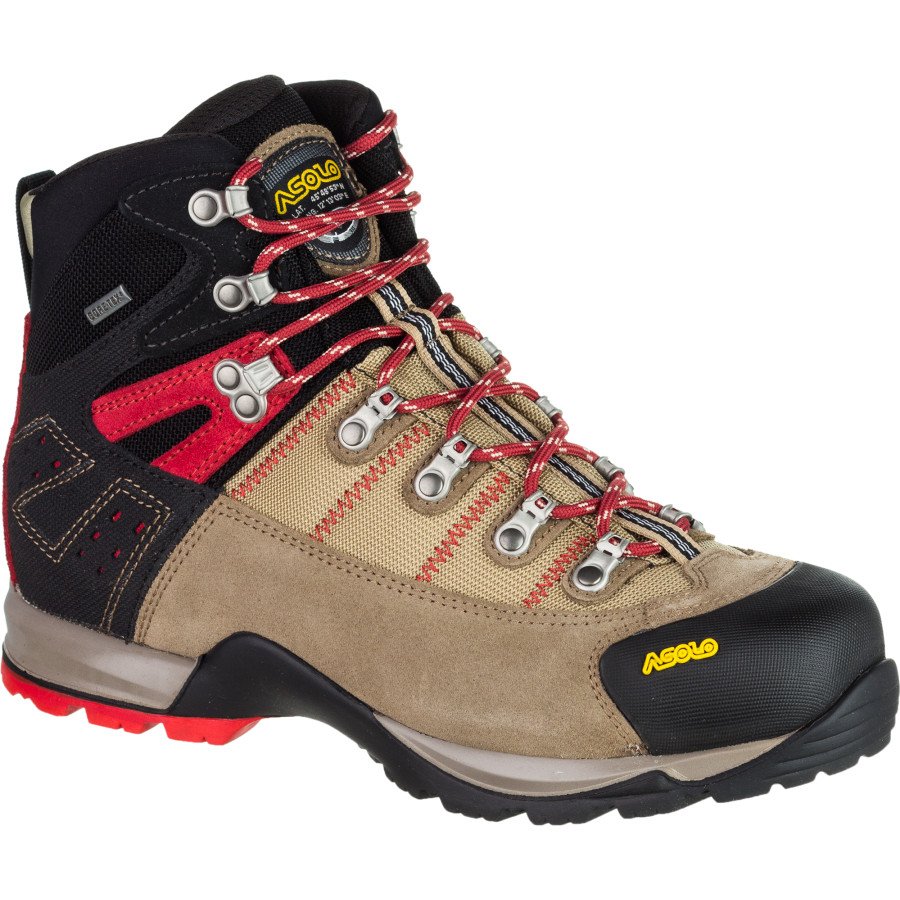
\includegraphics[height=6.7cm]{img/asolo}
\end{minipage}
\end{textblock*}
\end{frame}

\begin{frame}{So, we need a language}
\setstretch{1.2}
\begin{textblock*}{\framewidth-0.8cm}(0.0cm,1.5cm) % {block width} (coords)
\begin{minipage}{\textwidth}
  \centering
  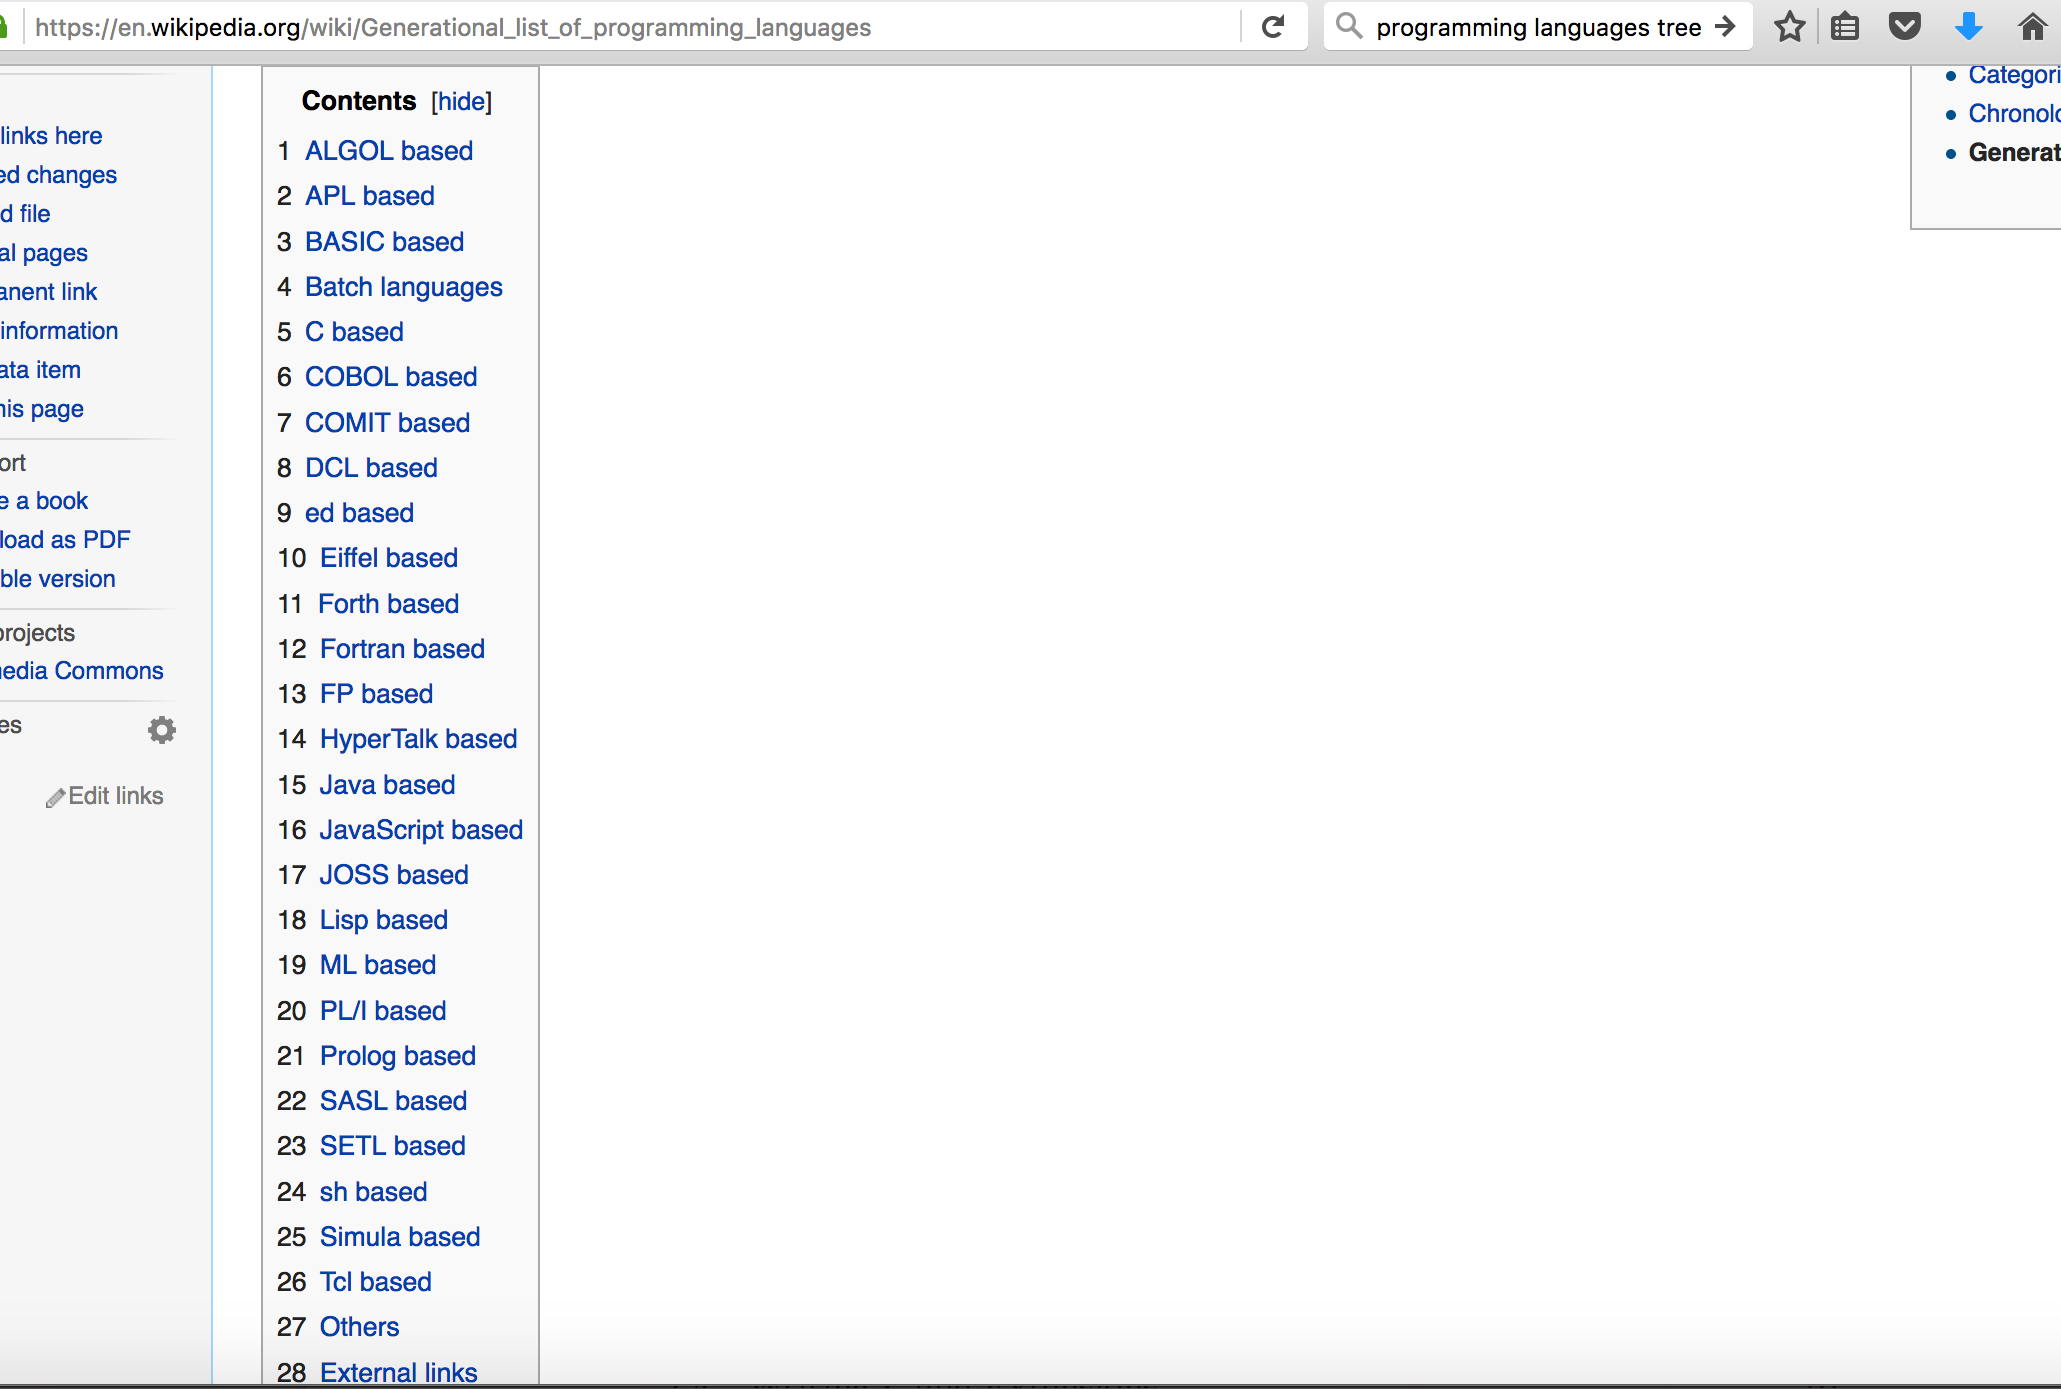
\includegraphics[height=6.7cm]{img/langs}
\end{minipage}
\end{textblock*}
\end{frame}

\begin{frame}{The obvious choice}
\setstretch{1.2}
\begin{textblock*}{\framewidth-0.8cm}(0.0cm,1.5cm) % {block width} (coords)
\begin{minipage}{\textwidth}
  \centering
  
\includegraphics[height=6.6cm]{img/vote-lisp}
\end{minipage}
\end{textblock*}
\end{frame}

\begin{frame}{Why Lisp?}
\setstretch{1.2}
\begin{textblock*}{\framewidth-0.8cm}(0.0cm,1.5cm) % {block width} (coords)
\begin{itemize}
  \item Homoiconicity
\end{itemize}
\end{textblock*}
\end{frame}

\begin{frame}{Why Lisp?}
\setstretch{1.2}
\begin{textblock*}{\framewidth-0.8cm}(0.0cm,1.5cm) % {block width} (coords)
\begin{itemize}
  \item Homoiconicity
  \item Macros
\end{itemize}
\end{textblock*}
\end{frame}

\begin{frame}{Why Lisp?}
\setstretch{1.2}
\begin{textblock*}{\framewidth-0.8cm}(0.0cm,1.5cm) % {block width} (coords)
\begin{itemize}
  \item Homoiconicity
  \item Macros
  \item Immutability (?)
\end{itemize}
\end{textblock*}
\end{frame}

\begin{frame}{Why Lisp?}
\setstretch{1.2}
\begin{textblock*}{\framewidth-0.8cm}(0.0cm,1.5cm) % {block width} (coords)
\begin{itemize}
  \item Homoiconicity
  \item Macros
  \item Immutability (?)
  \item Lambdas
\end{itemize}
\end{textblock*}
\end{frame}

\begin{frame}{But that was not too democratic, so...}
\setstretch{1.2}
\begin{textblock*}{\framewidth-0.8cm}(0.7cm,1.5cm) % {block width} (coords)
...what about Golang?
\begin{minipage}{\textwidth}
  \centering
  
\includegraphics[height=6.6cm]{img/hillary}
\end{minipage}
\end{textblock*}
\end{frame}

\begin{frame}{Unfortunately, Golang loses}
\setstretch{1.2}
\begin{textblock*}{\framewidth-0.8cm}(0.0cm,1.5cm) % {block width} (coords)
\begin{itemize}
  \item Way too modern (uses design ideas from 1970s while Lisp was born in 1958)
\end{itemize}
\end{textblock*}
\end{frame}

\begin{frame}{Unfortunately, Golang loses}
\setstretch{1.2}
\begin{textblock*}{\framewidth-0.8cm}(0.0cm,1.5cm) % {block width} (coords)
\begin{itemize}
  \item Way too modern (uses design ideas from 1970s while Lisp was born in 1958)
  \item Not functional enough (as in 'functional programming')
\end{itemize}
\end{textblock*}
\end{frame}

\begin{frame}{Unfortunately, Golang loses}
\setstretch{1.2}
\begin{textblock*}{\framewidth-0.8cm}(0.0cm,1.5cm) % {block width} (coords)
\begin{itemize}
  \item Way too modern (uses design ideas from 1970s while Lisp was born in 1958)
  \item Not functional enough (as in 'functional programming')
  \item Targets Java 1.2 and PHP 4.x market share (designed for apes not humans)
\end{itemize}
\end{textblock*}
\end{frame}

\begin{frame}{Runtime matters!}
\setstretch{1.2}
\begin{textblock*}{\framewidth-0.8cm}(0.0cm,1.5cm) % {block width} (coords)
\begin{itemize}
  \item Static linking is a must
\end{itemize}
\end{textblock*}
\end{frame}

\begin{frame}{Runtime matters!}
\setstretch{1.2}
\begin{textblock*}{\framewidth-0.8cm}(0.0cm,1.5cm) % {block width} (coords)
\begin{itemize}
  \item Static linking is a must
  \item Decent GC is a must
\end{itemize}
\end{textblock*}
\end{frame}

\begin{frame}{Runtime matters!}
\setstretch{1.2}
\begin{textblock*}{\framewidth-0.8cm}(0.0cm,1.5cm) % {block width} (coords)
\begin{itemize}
  \item Static linking is a must
  \item Decent GC is a must
  \item Resulting files should not be too big
\end{itemize}
\end{textblock*}
\end{frame}

\begin{frame}{Runtime matters!}
\setstretch{1.2}
\begin{textblock*}{\framewidth-0.8cm}(0.0cm,1.5cm) % {block width} (coords)
\begin{itemize}
  \item Static linking is a must
  \item Decent GC is a must
  \item Resulting files should not be too big
  \item Let's consider measureable things only
\end{itemize}
\end{textblock*}
\end{frame}

\begin{frame}{So, Lisps then}
\setstretch{1.2}
\begin{textblock*}{\framewidth-0.8cm}(0.0cm,1.5cm) % {block width} (coords)
\begin{itemize}
  \item Common Lisp
  \item Scheme
\end{itemize}
\begin{minipage}{\textwidth}
  \centering
  
\includegraphics[height=5.2cm]{img/lisplogo_256}
\end{minipage}
\end{textblock*}
\end{frame}

\begin{frame}{Common Lisp}
\setstretch{1.2}
\begin{textblock*}{\framewidth-0.8cm}(0.7cm,1.5cm) % {block width} (coords)
Statically linked file is over 30Mb (Golang does around 8Mb)
\begin{minipage}{\textwidth}
  \centering
  
\includegraphics[height=6.6cm]{img/fail1}
\end{minipage}
\end{textblock*}
\end{frame}

\begin{frame}{Scheme}
\setstretch{1.2}
\begin{textblock*}{\framewidth-0.8cm}(0.7cm,1.5cm) % {block width} (coords)
Is minimalist by design (way too minimalist I'd say)
\begin{minipage}{\textwidth}
  \centering
  
\includegraphics[height=6.6cm]{img/defer}
\end{minipage}
\end{textblock*}
\end{frame}

\begin{frame}{So, no boots then?}
\setstretch{1.2}
\begin{textblock*}{\framewidth-0.8cm}(0.7cm,1.5cm) % {block width} (coords)
\begin{minipage}{\textwidth}
  \centering
  
\includegraphics[height=6.9cm]{img/puss}
\end{minipage}
\end{textblock*}
\end{frame}

\begin{frame}{Nim to the rescue!}
\setstretch{1.2}
\begin{textblock*}{\framewidth-0.8cm}(0.7cm,1.5cm) % {block width} (coords)
Nim (formerly Nimrod)
\begin{minipage}{\textwidth}
  \centering
  
\includegraphics[width=11.3cm]{img/nim}
\end{minipage}
\end{textblock*}
\end{frame}

\begin{frame}{Nim: the good parts}
\setstretch{1.2}
\begin{textblock*}{\framewidth-0.8cm}(0.0cm,1.5cm) % {block width} (coords)
\begin{itemize}
  \item Strong typing
\end{itemize}
\end{textblock*}
\end{frame}

\begin{frame}{Nim: the good parts}
\setstretch{1.2}
\begin{textblock*}{\framewidth-0.8cm}(0.0cm,1.5cm) % {block width} (coords)
\begin{itemize}
  \item Strong typing
  \item Static typing
\end{itemize}
\end{textblock*}
\end{frame}

\begin{frame}{Nim: the good parts}
\setstretch{1.2}
\begin{textblock*}{\framewidth-0.8cm}(0.0cm,1.5cm) % {block width} (coords)
\begin{itemize}
  \item Strong typing
  \item Static typing
  \item Homoiconicity
\end{itemize}
\end{textblock*}
\end{frame}

\begin{frame}{Nim: the good parts}
\setstretch{1.2}
\begin{textblock*}{\framewidth-0.8cm}(0.0cm,1.5cm) % {block width} (coords)
\begin{itemize}
  \item Strong typing
  \item Static typing
  \item Homoiconicity
  \item Macro system (hygienic)
\end{itemize}
\end{textblock*}
\end{frame}

\begin{frame}{Nim: the good parts}
\setstretch{1.2}
\begin{textblock*}{\framewidth-0.8cm}(0.0cm,1.5cm) % {block width} (coords)
\begin{itemize}
  \item Strong typing
  \item Static typing
  \item Homoiconicity
  \item Macro system (hygienic)
  \item Immutability
\end{itemize}
\end{textblock*}
\end{frame}

\begin{frame}{Nim: the good parts}
\setstretch{1.2}
\begin{textblock*}{\framewidth-0.8cm}(0.0cm,1.5cm) % {block width} (coords)
\begin{itemize}
  \item Strong typing
  \item Static typing
  \item Homoiconicity
  \item Macro system (hygienic)
  \item Immutability
  \item Templates (generics)
\end{itemize}
\end{textblock*}
\end{frame}

\begin{frame}{Nim: runtime goodness}
\setstretch{1.2}
\begin{textblock*}{\framewidth-0.8cm}(0.0cm,1.5cm) % {block width} (coords)
\begin{itemize}
  \item Uses C as an IR
\end{itemize}
\end{textblock*}
\end{frame}

\begin{frame}{Nim: runtime goodness}
\setstretch{1.2}
\begin{textblock*}{\framewidth-0.8cm}(0.0cm,1.5cm) % {block width} (coords)
\begin{itemize}
  \item Uses C as an IR
  \item Per thread GC (as in Erlang)
\end{itemize}
\end{textblock*}
\end{frame}

\begin{frame}{Nim: runtime goodness}
\setstretch{1.2}
\begin{textblock*}{\framewidth-0.8cm}(0.0cm,1.5cm) % {block width} (coords)
\begin{itemize}
  \item Uses C as an IR
  \item Per thread GC (as in Erlang)
  \item Statically linked files < 1Mb (not stripped)
\end{itemize}
\end{textblock*}
\end{frame}

\begin{frame}{Project Kaldur}
\setstretch{1.2}
\begin{textblock*}{\framewidth-0.8cm}(0.0cm,1.5cm) % {block width} (coords)
\begin{itemize}
  \item Means 'cold' in Faroese
  \item Because it's quite cold now
  \item \href{https://github.com/alexclear/kaldur}{\color{blue}{https://github.com/alexclear/kaldur}}
\end{itemize}
\end{textblock*}
\end{frame}

\begin{frame}{Project Kaldur}
\setstretch{1.2}
\begin{textblock*}{\framewidth-0.8cm}(0.0cm,1.5cm) % {block width} (coords)
\begin{itemize}
  \item Is live at \href{http://185.37.61.240:5000}{\color{blue}{http://185.37.61.240:5000}}
  \item Has a TODO list on Github
  \item Has an issues list on Github
\end{itemize}
\end{textblock*}
\end{frame}

\begin{frame}{Conclusions}
\setstretch{1.2}
\begin{textblock*}{\framewidth-0.8cm}(0.0cm,1.5cm) % {block width} (coords)
\begin{itemize}
  \item TeX is great!
  \item Nim is great too!
  \item Flamegraphs are great!
  \item Linux is great!
  \item Open source projects are great!
\end{itemize}
\end{textblock*}
\end{frame}

\begin{frame}{Questions, please?}
\setstretch{1.2}
\begin{textblock*}{\framewidth-0.8cm}(0.0cm,1.5cm) % {block width} (coords)
\begin{itemize}
  \item Why FP?
  \item Why Linux?
  \item ...?
\end{itemize}
\end{textblock*}
\end{frame}

\begin{frame}{So long, and thanks for all the fish}
\setstretch{1.2}
\begin{textblock*}{\framewidth-0.8cm}(0.0cm,1.5cm) % {block width} (coords)
\begin{itemize}
  \item \href{mailto:achistyakov@dataart.com}{\color{blue}{achistyakov@dataart.com}}
  \item \href{https://telegram.me/lhommequipleure}{\color{blue}{https://telegram.me/lhommequipleure}}
\end{itemize}
\end{textblock*}
\end{frame}

\end{document}